% !TEX root = ../main.tex
\section{Representation Learning and Construction}
\label{sec:representation}

The choice of denoising representation determines both what a continuous diffusion model must learn and how its outputs can be converted back to language. Pretrained networks offer a useful starting point: ELF uses contextual embeddings from a bidirectional T5 encoder \citep{elf}, while work on image generation shows how pretrained visual representations can guide diffusion. REPA aligns denoiser features with clean visual features \citep{repa}; Semantic-First Diffusion (SFD) and Latent Forcing instead augment the generated state with semantic representations derived from pretrained vision encoders \citep{sfd,latentforcing}. These successes motivate using a powerful model's output features, but leave open which layers and compression objectives are most suitable for reasoning in language.

We use \textbf{teacher-forced hidden activations of Qwen3-4B-Instruct-2507} \citep{qwen2507}. Qwen provides a strong reasoning model: our autoregressive evaluation achieves 92.19\% on GSM8K (Appendix~\ref{app:representationdiagnostics}). Given a question and its complete reference solution, all token activations can be computed in one teacher-forced forward pass. Although these activations come from a causal language model, the generator trained on them need not be causal. Our bidirectional denoiser generates the complete sequence of answer latents jointly, making the teacher's representation available to a different generative process.

A useful representation must satisfy two requirements: \textbf{decodability}, retaining the information needed to recover a solution, and \textbf{generatability}, admitting effective conditional denoising within the available model capacity and training budget. Strong decoding alone does not establish the second property. In particular, the effectiveness of final visual-encoder features in prior work does not determine the best depth to use in an autoregressive language model. We describe our learned, multilayer construction in Section~\ref{sec:representationconstruction}, then examine layer selection and projection learning in Section~\ref{sec:representationablations}. Figure~\ref{fig:representationcomparison} summarizes the resulting differences in reasoning performance.

% !TEX root = ../main.tex
\begin{figure}[htbp]
\centering
\begin{minipage}[c]{.55\linewidth}
\centering
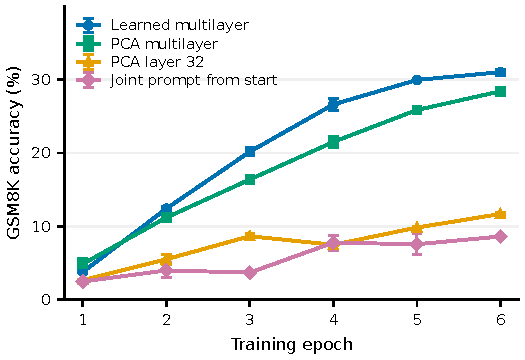
\includegraphics[width=\linewidth]{figures/representation_shared2_sd.pdf}
\end{minipage}\hfill
\begin{minipage}[c]{.43\linewidth}
\centering
% !TEX root = ../main.tex
% Generated from exact per-seed counts; parentheses are sample SD, ddof=1.
\begingroup
\small
\setlength{\tabcolsep}{3pt}
\renewcommand{\arraystretch}{1.25}
\begin{tabular}{@{}lr@{}}
\toprule
Variant & Accuracy (\%) \\
\midrule
Learned, 16/24/32 & \textbf{30.76} {\scriptsize (0.39)} \\
PCA, 16/24/32 & 28.43 {\scriptsize (0.19)} \\
PCA, layer 32 & 11.20 {\scriptsize (0.56)} \\
Epoch 0 learned prompt encoder & 8.70 {\scriptsize (0.33)} \\
\bottomrule
\end{tabular}
\endgroup

\end{minipage}
\caption{\textbf{Representation and conditioning choices change reasoning performance.} ELF-B on GSM8K with shared $t=\tau^2$, 32 steps, and ELF EMA $0.999$. \textbf{Left:} learning curves over seeds 42/123 (bars: seed SD). \textbf{Right:} epoch-six means over seeds 42/123/456/789 (parentheses: seed SD); reporting conventions are in Appendix~\ref{app:experimentdetails}. All latents are whitened and 1,024-dimensional. The first three variants use frozen Qwen prompt activations. The fourth uses learned multilayer answer latents and a randomly initialized prompt encoder trained jointly from epoch zero (prompt EMA $0.999$). The epoch-six ordering persists with the identity clock $t=\tau$ (Appendix~\ref{app:representationclock}).}
\label{fig:representationcomparison}
\end{figure}


\subsection{Learning compact, teacher-predictive representations}
\label{sec:representationconstruction}

\paragraph{Teacher features and latent construction.}
Let $q$ denote the question prefix, $a=(a_1,\ldots,a_T)$ its solution, and $h_j^{(\ell)}\in\R^{2560}$ the frozen teacher's post-block residual at answer position $j$. The native causal mask gives $h_j^{(\ell)}=h_\psi^{(\ell)}(q,a_{\leq j})$; extracting all these states requires one forward pass over $(q,a)$. For $\mathcal S=\{16,24,32\}$, we learn a linear encoder $E_\ell\in\R^{2560\times d_\ell}$ and form
\begin{equation}
 z_j^{(\ell)}=(h_j^{(\ell)}-\mu_\ell)E_\ell,
 \qquad
 z_j=\big[z_j^{(16)},z_j^{(24)},z_j^{(32)}\big]\in\R^{1024},
 \label{eq:representationencoding}
\end{equation}
where $(d_{16},d_{24},d_{32})=(256,256,512)$ and $\mu_\ell$ is the training assistant-token mean. The same maps encode question-prefix states for the initial flow-training stage. Causal feature extraction ensures that these question states are independent of the subsequent answer. Once learned, the answer representation remains fixed throughout flow training and NFT.

\paragraph{Learning through the teacher's predictions.}
We train the encoders to preserve the teacher's predictive behavior, as illustrated in the first column of Figure~\ref{fig:pipelineoverview}. For each selected layer, a trainable linear reconstruction decoder $D_\ell\in\R^{2560\times d_\ell}$ maps latents back to the original hidden width:
\begin{equation}
 \widehat h_j^{(\ell)}=\mu_\ell+z_j^{(\ell)}D_\ell^\top.
 \label{eq:representationreconstruction}
\end{equation}
We replace the assistant-content activations at layer $\ell$ by these reconstructions and run the remaining frozen Qwen blocks, final normalization, and vocabulary head. Write $p_j^{\mathrm{teacher}}$ for the unmodified teacher's next-token distribution and $p_{\ell,j}^{\mathrm{recon}}$ for this intervened branch. The representation objective is full-vocabulary categorical cross-entropy:
\begin{equation}
 \mathcal L_{\mathrm{repr}}
 =\sum_{\ell\in\mathcal S}\E_{q,a,j}
 \left[-\sum_{v\in\mathcal V}p_j^{\mathrm{teacher}}(v)
 \log p_{\ell,j}^{\mathrm{recon}}(v)\right].
 \label{eq:representationloss}
\end{equation}
The teacher target is detached, while gradients through the frozen suffix train $E_\ell$ and $D_\ell$. Each layer is intervened on independently; prompt and control-token states remain unchanged. Scored positions predict the following assistant-content token. Thus the objective asks whether compression preserves the teacher's decisions, rather than requiring an accurate reconstruction of every hidden-state coordinate. The reconstruction decoders and Qwen suffixes are used to learn the representation; generation later uses ELF's shared backbone and token head.

\paragraph{Fixing the latent geometry.}
The reconstruction map admits changes of latent scale that can be absorbed by its decoder. We fix this freedom before applying isotropic diffusion noise. With regularized assistant-token covariance $\widetilde C_\ell$, we parameterize
\begin{equation}
 Q_\ell=\operatorname{qf}(R_\ell),\qquad
 E_\ell=\widetilde C_\ell^{-1/2}Q_\ell,\qquad
 E_\ell^\top\widetilde C_\ell E_\ell=I_{d_\ell},
 \label{eq:representationwhitening}
\end{equation}
where $\operatorname{qf}$ is a differentiable thin QR factorization and $R_\ell$ is trainable. We initialize from the leading PCA directions and then optimize Eq.~\eqref{eq:representationloss}, allowing $D_\ell$ to adapt freely. This maintains a nondegenerate coordinate scale while the subspace changes. Whitening acts within each layer group; correlations between groups remain. Appendix~\ref{app:representationimplementation} specifies covariance regularization and initialization.

\subsection{Which representation should be denoised?}
\label{sec:representationablations}

We compare ELF-B models trained for six epochs on the same 2.43M-row GSM8K training population, with the same ELF initialization, optimization batch, and synchronous training clocks. All representations have width 1,024 and use covariance whitening. The main comparisons use original Qwen question conditioning, holding the representation fixed during ELF training. We evaluate with a common $t=\tau^2$ clock, 32 denoising steps, and ELF EMA $0.999$. The fourth arm in Figure~\ref{fig:representationcomparison} retains the learned multilayer answer representation but learns its prompt encoder jointly from initialization; it provides context for the separate question of when to learn conditioning.

\paragraph{A deep layer is readily decodable, yet difficult to generate from alone.}
A same-position token probe recovers \textbf{99.37\%} of held-out assistant tokens from clean layer-32 activations. Layers 16 and 24 also give high recovery, at 99.63\% and 99.53\%, respectively (Appendix~\ref{app:representationdiagnostics}). These probes use a learned 1,024-dimensional bottleneck on full teacher activations, so they establish clean-token decodability rather than the reconstruction accuracy of the fixed PCA encoders. Nevertheless, training diffusion on the top 1,024 whitened PCA coordinates of layer 32 yields only \textbf{11.20\%} GSM8K accuracy at epoch six. Here layer 32 is a deep-layer control, not Qwen's final block: the teacher has 36 blocks. The combination of easy clean-token recovery and weak downstream generation motivates looking beyond decoding fidelity when choosing the latent space.

\begin{figure}[htbp]
\centering
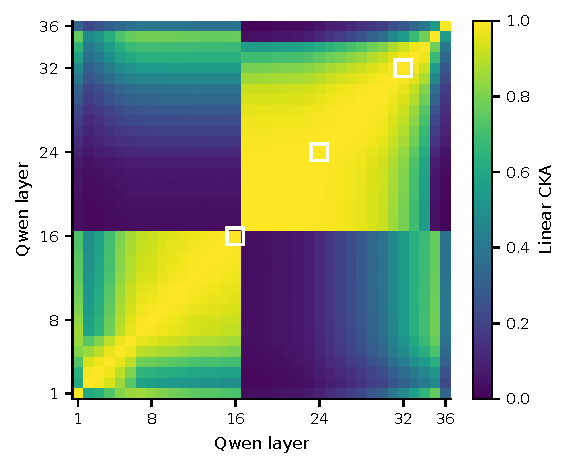
\includegraphics[width=.53\linewidth]{figures/cka.pdf}
\caption{\textbf{Representation structure across Qwen depth.} Linear CKA between teacher-forced post-block activations; white markers identify layers 16, 24, and 32. The transition after layer 16 motivates including it, while layers 24 and 32 sample deeper representations at regular intervals. Activations are pooled within eight relative-position bins and compared across 8,192 problems with equal weight per problem.}
\label{fig:representationcka}
\end{figure}

\paragraph{Combining representations across depth.}
Figure~\ref{fig:representationcka} uses centered kernel alignment (CKA; \citealp{cka}) to examine the teacher's layer structure. A pronounced change after layer 16 suggests retaining a representation at that boundary. We then choose layers 24 and 32 as regularly spaced deeper features. This is a structural motivation for the triplet, rather than an exhaustive search over layer combinations. With PCA held fixed as the projection method, replacing the layer-32-only representation by 256/256/512 coordinates from layers 16/24/32 raises epoch-six accuracy from \textbf{11.20\% to 28.43\%}, a gain of 17.23 percentage points (paired 95\% problem-bootstrap interval $[15.50,18.97]$). The multilayer PCA model also leads at every evaluated epoch. This decomposition supplies distinct feature groups for the asynchronous denoising framework: representation construction creates the opportunity to assign different dynamics to information extracted at different depths.

\paragraph{Learning a predictive subspace improves on variance preservation.}
PCA retains directions of largest activation variance, minimizing Euclidean reconstruction error at a fixed rank. High variance, however, need not identify the directions most important to the teacher's token predictions or easiest for a diffusion model to use. Our linear encoder--decoder construction offers an efficient way to adapt the subspace to the former criterion using the frozen teacher's own predictions. Holding layers and dimensions fixed, learning the projectors raises epoch-six accuracy from \textbf{28.43\% to 30.76\%}, a gain of 2.33 points ($[0.87,3.81]$). It also leads multilayer PCA from epoch two onward. The ordering persists with the identity inference clock (Appendix~\ref{app:representationclock}). Together, the comparisons support selecting representations for their downstream generative utility as well as their information content: both the depths represented and the compression objective matter within a matched training budget.
